%課題研究レジュメテンプレート ver. 1.2

\documentclass[uplatex]{jsarticle}
\usepackage[top=20mm,bottom=20mm,left=20mm,right=20mm]{geometry}
\usepackage[T1]{fontenc}
\usepackage{txfonts}
\usepackage{wrapfig}
\usepackage[expert,deluxe]{otf}
\usepackage[dvipdfmx,hiresbb]{graphicx}
\usepackage[dvipdfmx]{hyperref}
\usepackage{pxjahyper}
\usepackage{secdot}

\makeatletter
  \renewcommand{\section}{%
    \if@slide\clearpage\fi
    \@startsection{section}{1}{\z@}%
    {\Cvs \@plus.5\Cdp \@minus.2\Cdp}% 前アキ
    {.5\Cvs \@plus.3\Cdp}% 後アキ
    %{\normalfont\Large\headfont\raggedright}}
    {\normalfont\raggedright}}

  \renewcommand{\subsection}{\@startsection{subsection}{2}{\z@}%
    {\Cvs \@plus.5\Cdp \@minus.2\Cdp}% 前アキ
    {.5\Cvs \@plus.3\Cdp}% 後アキ
    %{\normalfont\large\headfont}}
    {\normalfont}}

  \renewcommand{\subsubsection}{\@startsection{subsubsection}{3}{\z@}%
    {\Cvs \@plus.5\Cdp \@minus.2\Cdp}%
    {\z@}%
    %{\normalfont\normalsize\headfont}}
    {\normalfont}}
\makeatother
%ここから上を編集する必要はない.





\title{\vspace{-14mm}社会実装を目的とした3学科合同介護機器開発プロジェクト}
\author{PMコース 矢吹研究室 1442069 氏名 須山 武弘}
\date{}%日付を入れる必要はない.
\pagestyle{empty}%ページ番号は振らない.
\begin{document}
\maketitle





\section{研究の背景}
少子高齢化が進み,健康寿命が短くなっている現在,介護業界はこれから重要となり,需要も増加傾向にある業界である\cite{hakusyo}.実際に特別養護老人ホームの入所申込者数(待機者数)は09年~14年の5年間で10万人増加している.待機者数増加の要因として考えられるのは,1947年~1949年に生まれた団塊世代の人たちが徐々に介護サービスを必要としてきているからである\cite{minnano}.

介護職員は賃金,労働時間,体力的,精神的な負担が大きい.これらの要因から介護現場は厳しい労働環境であり,離職率が高い.さらに平成26年時点で介護分野における有効求人倍率が2倍を超えている状況であるため,増える介護の需要に介護職員の人数が追いついていないといえる\cite{jinzai}.介護現場の人材不足を解消するには介護のオートメーション化や外国人労働者の雇用,介護職員の負担軽減が必要であると考えられる.

プロジェクトマネジメント学科,未来ロボティクス学科,デザイン科学科(以下,3学科)の3学科合同のチームを編成し,介護職員の負担を軽減するために使用でき,理想の介護であるその人らしい生活をサポートできる介護機器の開発プロジェクトを遂行した.さらに,この介護機器開発プロジェクトは,製品開発のみならず,実際に社会に売り出すことのできるところまで考える社会実装を目的とした活動である.

専門分野の異なる3学科合同で行っているため,プロジェクトマネジメント学科内だけで行っている演習とは違い,それぞれの専門分野を活かし,それぞれの意見をまとめプロジェクトを成功へ導くマネジメントが必要である.

\section{研究の目的}
現在の介護職員に対する負担が大きく,人材不足である介護現場を技術で支えるため,開発した製品の社会実装を目的としたSI-LAB(Society Implementation Laboratory)の活動を通して,介護機器を開発することが目的である.

製品開発をするにあたって3学科の専門分野を活かしたマネジメント手法を実施し,プロジェクトを成功へ導く.

\section{プロジェクトマネジメントとの関連}
SI-LABの活動を通してプロジェクトマネジメント学科以外の他学科の特徴を踏まえたプロジェクトマネジメント及び,人的資源の適切な配分を行う.


\section{研究の方法}

3学科合同の4人チームを編成し,介護現場の問題点を現地調査などから発見する.その問題点を解決,補助するための製品開発プロジェクトを2016年7月~17年2月にかけて表1のように遂行し,適宜,適切なマネジメント手法を実施する.

\begin{table}[h]
  \caption{チーム編成から製品の製作までの期間とタスク}
  \label{table:data_type}
  \centering
  \begin{tabular}{ l l }
\hline
期間 & タスク \\ \hline
    7月~9月 & チームを編成.介護施設を訪問し,問題点を話し合う.問題点を解決,補助できる製品を提案する. \\
    9月~10月  & キャンパスベンチャーグランプリ(以下,CVG)へ応募書類の作成及び,ビジネスプランの作成をする. \\
    11月  & CVGの書類選考を通過.予選へ向けてのプレゼンをする. \\
12月~1月  & 実際に使える製品の製作.機構の検討をする. \\
1月~2月 &製品の製作.介護関係者へ向けてのプレゼンの準備をする. \\ \hline
  \end{tabular}
\end{table}

\section{現在の進捗状況}

介護現場の調査へ出向き,問題点を洗い出し,メンバーでブレーンストーミングやKJ法を用いた結果,トイレ介助が介護現場の大きな負担になっている事が判明した.その点からトイレ介助の際に介護職員及び,要介護者をサポートする機器を考案した.考案した製品が図1である.

大学生を対象としたビジネスコンテストであるCVGに製品と合わせてビジネスプランを作成し,応募した.その結果,書類選考を通過し,東京大会の予選にてプレゼンを行った.

これまでの活動で,ビジネスプランの作成及び,ガントチャートによるスケジュール管理,人的資源管理はプロジェクトマネジメント学科,製品のデザインはデザイン科学科,機構及び,製品の強度は未来ロボティクス学科が担当している.

\begin{figure}[htbp]
  \begin{center}
    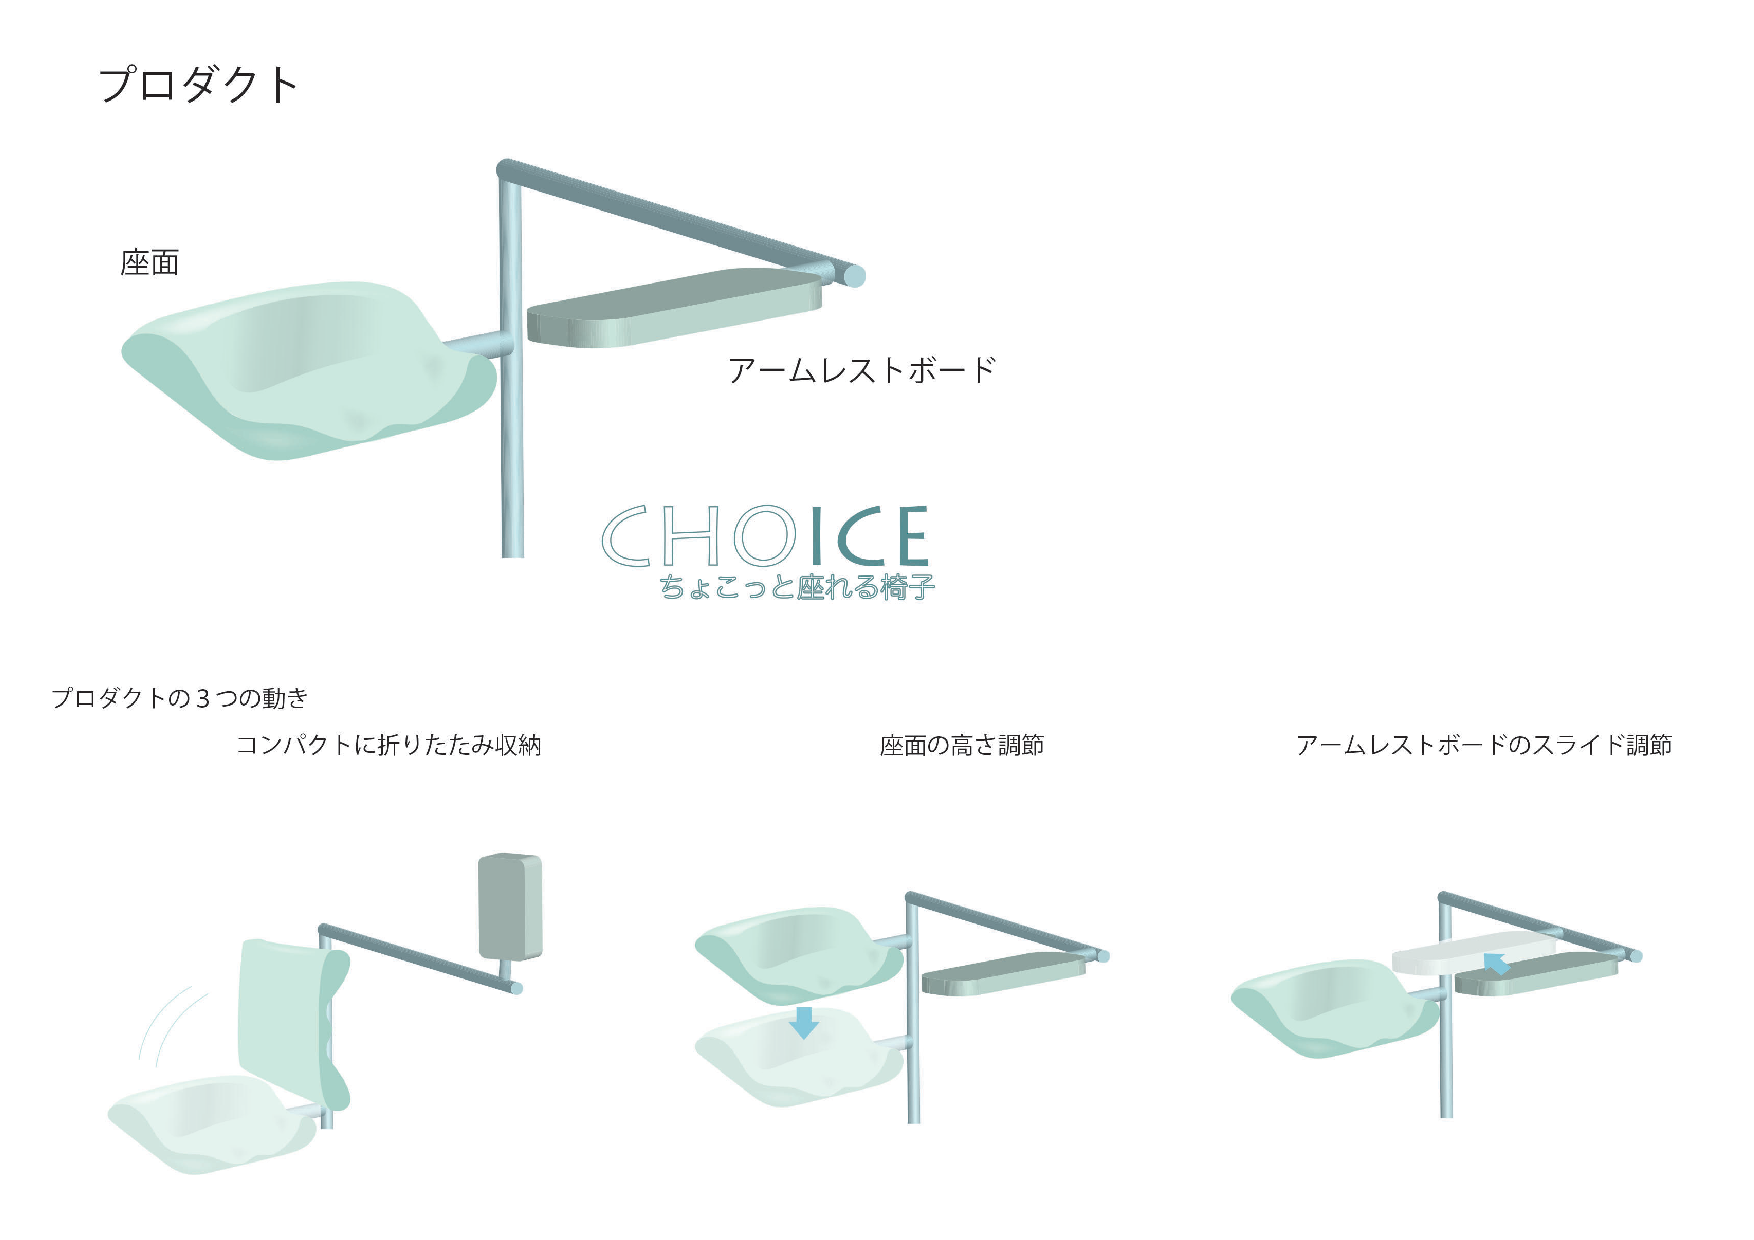
\includegraphics[clip,width=12cm]{images.pdf}
    \caption{開発した製品}
    \label{サンプル図}
  \end{center}
\end{figure}


\section{今後の計画}

以下のように研究を進めていく.

\begin{itemize}
\item 専門家であるプロの企業様に協力を仰ぎながら製品を試作をする.
\item 試作品を使って安全性や使い勝手などを検証する.
\item プロジェクト終結プロセスへ向けてプロジェクトのまとめをする.
\end{itemize}

\bibliographystyle{junsrt}
\bibliography{biblio}%「biblio.bib」というファイルが必要.

\end{document}
